% !TeX program = pdflatex
\documentclass{iutbscthesis}

\addbibresource{citations.bib}

% Title
\title{Orthogonal Defect Classification on Defects4J Using an LLM-Driven Scientific Approach}

% Authors
\addauthor{Hasin Mahtab Alvee}{210042174}
\addauthor{Mohammad Nahiyan Kabir}{210042168}
\addauthor{Md. Sakib Hossain}{210042133}

% Supervisor
\supervisor{Lutfun Nahar Lota}{Assistant Professor}{Department of Computer Science and Engineering}

% Co-supervisor
\addcosupervisor{Ishmam Tashdeed}{Lecturer}{Department of Computer Science and Engineering}

% Department
\department{Department of Computer Science and Engineering}

% Program
\program{BACHELOR OF SCIENCE IN COMPUTER SCIENCE AND ENGINEERING}

% Defense date
\defensedate{XX}{Month}{2026}

\begin{document}

%-------------------------- FRONT MATTER --------------------------%

\coverpage
\pagenumbering{roman}
\titlepage
\declarationofcandidate

\dedicatedto{our families, friends, and mentors who supported us throughout this journey}

\tableofcontents
\listoffigures
\listoftables

\clearpage

\begin{abbreviations}
    \abbr{APR}{Automated Program Repair}
    \abbr{API}{Application Programming Interface}
    \abbr{CFG}{Control Flow Graph}
    \abbr{CLI}{Command Line Interface}
    \abbr{CoT}{Chain-of-Thought}
    \abbr{D4J}{Defects4J}
    \abbr{DFG}{Data Flow Graph}
    \abbr{LLM}{Large Language Model}
    \abbr{ML}{Machine Learning}
    \abbr{NLP}{Natural Language Processing}
    \abbr{ODC}{Orthogonal Defect Classification}
    \abbr{SDLC}{Software Development Life Cycle}
    \abbr{SVM}{Support Vector Machine}
\end{abbreviations}

\begin{acknowledgement}
We would like to express our sincere gratitude to our supervisor, Lutfun Nahar Lota, and our co-supervisor, Ishmam Tashdeed, for their continuous guidance and support throughout this research. Their expertise and encouragement helped shape this work from concept to completion.

We are also grateful to the Network and Data Analysis Group (NDAG) Lab at IUT for providing the research environment and resources that made this thesis possible.

Finally, we thank our families for their patience and support during the many long hours that went into this research.
\end{acknowledgement}

\begin{abstract}
Bug classification plays a key role in software quality assurance, helping developers understand defect patterns and improve their development processes. However, no study has ever fully labeled all bugs in the Defects4J benchmark dataset using a principled, root-cause taxonomy. Existing classification efforts cover only small subsets (50 to 488 bugs), rely on structural taxonomies that describe how bugs look rather than why they occur, or depend on post-fix code that is not available during real-world triage. This thesis presents an automated pipeline that classifies Defects4J bugs into seven Orthogonal Defect Classification (ODC) defect types using Large Language Model (LLM) reasoning guided by a scientific debugging protocol. The pipeline collects multi-modal evidence from Defects4J artifacts, including bug reports, stack traces, failing tests, and source code snippets, and constructs structured prompts that combine the ODC taxonomy with Zeller's scientific debugging methodology. Classification operates in two evidence modes: pre-fix (symptoms only) and post-fix (with the actual code fix), enabling a built-in evaluation through comparison. Preliminary analysis of 34 bug pairs across 17 projects shows 73.5\% strict type match, 94.1\% top-2 match, and 97.1\% family match between the two modes, demonstrating robust classification consistency that aligns with the expected 20 to 30\% human disagreement ceiling reported in ODC literature.
\end{abstract}

%-------------------------- MAIN BODY --------------------------%
\pagenumbering{arabic}

% ================================================================
% CHAPTER 1: INTRODUCTION
% ================================================================
\chapter{Introduction}

Software bugs are an unavoidable part of the development process. Even the most carefully written programs contain defects that cause unexpected behavior, crashes, or incorrect results. Identifying these bugs is only the first step. Understanding what kind of bug it is, why it happened, and how it should be fixed is equally important for improving software quality over time \cite{catolino2019not}.

In practice, developers spend a significant portion of their time triaging and debugging reported issues. Bug categorization helps make this process more efficient by grouping defects into meaningful categories that guide debugging strategies and resource allocation \cite{andrade2025empirical}. Early prediction of a bug's category from its report helps teams prioritize work before even looking at the code \cite{hirsch2022using}. Structured categorization also provides actionable measurements that managers and developers can use to improve their processes \cite{chillarege1992odc}.

\section{Defects4J: The Benchmark Dataset}

Defects4J is a curated database of real, reproducible Java bugs paired with developer-written patches and regression test suites \cite{just2014defects4j}. It has grown to include over 864 active bugs across 17 Java projects and serves as the standard benchmark for empirical software engineering research, including fault localization, automated program repair, and testing studies \cite{rafi2024revisiting, durieux2018automatic}.

Each bug in Defects4J comes with a rich set of artifacts: the original bug report, triggering tests that expose the bug, the buggy source code, the fixed source code, and code diffs showing exactly what changed. These artifacts make Defects4J particularly well suited for automated analysis because they provide multiple perspectives on each defect.

\section{Motivation}

Despite the widespread use of Defects4J in software engineering research, no study has ever fully classified all of its bugs using a principled, root-cause taxonomy. Existing classification efforts fall into three categories, each with significant limitations.

First, structural approaches like the work of \textcite{vanderspuy2025anatomy} classify bugs based on control-flow and data-flow graph representations. While this covers 488 bugs across 7 projects, it captures how bugs manifest syntactically rather than why they exist semantically.

Second, patch-level taxonomies like the Defects4J Dissection by \textcite{sobreira2018dissection} classify repair actions for 395 bugs from an older version of the dataset. This describes fix patterns but does not identify root causes.

Third, small-sample inspections like the work of \textcite{xuan2017better} manually analyze 50 randomly selected bugs. While detailed, this approach does not scale.

None of these approaches apply a semantic, root-cause taxonomy to the full dataset. This gap motivates the need for an automated, scalable classification approach that goes beyond surface-level structural patterns.

\section{Research Objectives}

This thesis addresses the following four research objectives:

\begin{enumerate}
    \item[\textbf{RO-1:}] Build an automated pipeline that classifies Defects4J bugs into ODC defect types using LLM reasoning guided by structured scientific debugging.
    \item[\textbf{RO-2:}] Collect bug evidence in two modes, pre-fix (symptoms only) and post-fix (with the actual code fix), mapping Defects4J artifacts to ODC opener and closer attributes.
    \item[\textbf{RO-3:}] Apply Zeller's scientific debugging methodology as an LLM prompting strategy to produce explainable, step-by-step classifications.
    \item[\textbf{RO-4:}] Design a 4-tier evaluation framework that compares pre-fix and post-fix classifications using strict match, top-2 match, family match, and Cohen's Kappa.
\end{enumerate}

\section{Contributions}

The main contributions of this thesis are:

\begin{itemize}
    \item A fully automated, end-to-end pipeline that collects multi-modal evidence from Defects4J and produces machine-readable ODC classifications with full reasoning traces.
    \item A dual-mode evidence collection system (pre-fix and post-fix) that mirrors ODC's opener/closer model and enables built-in evaluation.
    \item A structured prompting approach that encodes the ODC taxonomy and Zeller's scientific debugging protocol into LLM prompts, producing explainable classifications.
    \item A 4-tier evaluation framework that respects the inherent ambiguity in defect classification rather than demanding perfect agreement.
\end{itemize}

\section{Report Organization}

The rest of this report is organized as follows. Chapter 2 reviews the related literature on Defects4J classification, LLM-based bug categorization, and the ODC framework. Chapter 3 defines the research gap and problem statement. Chapter 4 describes the proposed methodology in detail. Chapter 5 explains the experimental design and data collection approach. Chapter 6 presents the preliminary results and analysis. Chapter 7 provides the project timeline. Finally, Chapter 8 concludes the report with a summary, limitations, and future work.


% ================================================================
% CHAPTER 2: RELATED WORKS / LITERATURE REVIEW
% ================================================================
\chapter{Related Works}

This chapter reviews the existing literature that forms the foundation of our research. We organize the review around four themes: existing attempts at classifying Defects4J bugs, the emergence of LLM-based defect classification, the challenge of choosing the right taxonomy, and the Orthogonal Defect Classification framework that our pipeline adopts.

\section{Existing Defects4J Classification Attempts}

Several studies have attempted to classify bugs in the Defects4J dataset, each using a different approach and covering a different subset of the data.

The most recent effort is by \textcite{vanderspuy2025anatomy}, who manually classified 488 Defects4J bugs into six control-flow and two data-flow categories based on their graph representations. This structural approach reveals how bugs change the program's execution paths, but it does not explain the semantic root cause of the defect. For example, a missing null check and a completely absent feature might both appear as similar control-flow changes, even though they represent fundamentally different types of problems.

\textcite{sobreira2018dissection} performed an earlier classification of 395 bugs from Defects4J version 1.2, focusing on repair actions and repair patterns. Their work found that 43\% of patches involve conditional block changes. While this provides useful information about fix patterns, it describes what developers changed rather than why the bug existed in the first place.

\textcite{xuan2017better} conducted a manual inspection of 50 randomly selected Defects4J bugs, identifying fixability patterns and assessing the quality of test-suite artifacts. While this small-sample study reveals important details, the authors themselves acknowledge the limited external validity of examining only 50 bugs.

These three studies collectively represent structural classification, patch-level classification, and small-sample inspection. None of them applies a semantic, root-cause taxonomy like ODC to the full Defects4J dataset.

\section{LLM-Based Defect Classification}

Recent research has shown that Large Language Models can effectively classify software defects when given appropriate prompting strategies.

\textcite{colavito2024llm} demonstrated that LLMs can classify issue reports (closely related to bug reports) with reasonable accuracy, validating the basic hypothesis that LLMs are suitable for defect classification tasks. \textcite{koyuncu2025exploring} extended this by using prompt engineering techniques, including few-shot prompting, to achieve fine-grained bug report categorization. Their work is the most directly relevant prior study to our approach.

Chain-of-thought prompting has also proven effective for structured classification tasks. \textcite{nong2024cot} showed that CoT prompting improves LLM classification accuracy by over 500\% on vulnerability analysis tasks, suggesting that structured reasoning significantly helps LLMs perform better on classification problems.

\textcite{gao2024rcegen} demonstrated that LLMs can generate structured, ODC-aligned root cause explanations from bug reports and stack traces, showing that LLMs can reason about semantic defect categories when provided with appropriate guidance.

Compared to traditional machine learning approaches, LLMs offer a key advantage: they are code-aware. Earlier automated ODC systems using SVM and Naive Bayes classifiers achieved only 77 to 82\% accuracy and struggled with sparse text inputs \cite{huang2011autoodc, thung2012automatic}. LLMs overcome these limitations because they can reason about code structure, test semantics, and error messages simultaneously, without requiring labeled training data.

\section{The Taxonomy Problem}

While LLMs show promise for defect classification, using them without a structured taxonomy leads to unreliable results.

\textcite{gao2024rcegen} noted that LLMs hallucinate heavily when classifying bugs without concrete stack traces or a guiding taxonomy. Without standardization, different LLM runs produce different category labels for the same bug \cite{koyuncu2025exploring}. Machine learning-based bug classification studies also suffer from a proliferation of incompatible taxonomies, making it impossible to compare results across studies \cite{andrade2025empirical}. Classification without a principled framework produces vague labels with no operational value \cite{thung2012automatic}.

This problem motivates the need for a well-established, mathematically rigorous taxonomy to constrain and guide LLM outputs. That taxonomy is Orthogonal Defect Classification.

\section{Orthogonal Defect Classification (ODC)}

ODC was introduced by \textcite{chillarege1992odc} as a framework for classifying software defects using orthogonal (independent) attributes that provide actionable, in-process measurements. The framework defines eight attributes organized into two phases:

\begin{itemize}
    \item \textbf{Opener attributes} (recorded when the defect is found): Activity, Trigger, and Impact. These capture the discovery context: what was being done, what condition exposed the defect, and what effect it had.
    \item \textbf{Closer attributes} (recorded when the defect is fixed): Defect Type, Target, Qualifier, Age, and Source. These capture the repair context: what kind of mistake it was, where it was located, and how it manifested.
\end{itemize}

The central attribute for our work is the Defect Type, which classifies the root cause mechanism into seven categories for Design/Code targets: Algorithm/Method, Assignment/Initialization, Checking, Timing/Serialization, Function/Class/Object, Interface/O-O Messages, and Relationship. These seven types are grouped into two families: Control and Data Flow (the first four) and Structural (the last three).

ODC remains actively used in modern research. \textcite{pan2024understanding} applied ODC to classify defects in LLM-generated code in 2024, demonstrating that the taxonomy generalizes beyond human-written software. The official ODC v5.2 specification from IBM \cite{ibm2013odc} continues to serve as the reference standard for the framework.

\section{Summary}

The literature reveals a clear gap: no study has applied a semantic, root-cause taxonomy like ODC to the full Defects4J dataset using automated classification. Existing work either covers small subsets, uses structural-only taxonomies, or requires labeled training data that Defects4J lacks. LLMs offer a viable path forward, but they need a structured taxonomy to produce consistent, actionable results. Our thesis addresses this gap by combining LLM reasoning with ODC constraints and a scientific debugging protocol.


% ================================================================
% CHAPTER 3: PROBLEM STATEMENT
% ================================================================
\chapter{Problem Statement}

This chapter defines the specific research gap that our thesis addresses and formally states the problem we aim to solve.

\section{Limitations of Existing Approaches}

Current attempts at classifying Defects4J bugs suffer from five critical limitations:

\begin{enumerate}
    \item \textbf{Coverage Gap:} No study has fully labeled all 864+ Defects4J bugs. Existing work covers only 50 to 488 bugs \cite{sobreira2018dissection, vanderspuy2025anatomy, xuan2017better}.
    \item \textbf{Structural-Only Taxonomy:} Control-flow and data-flow graph approaches capture how bugs manifest syntactically, not why they exist semantically \cite{vanderspuy2025anatomy}.
    \item \textbf{Patch-Level Focus:} Repair-action classification describes fix patterns, not the underlying root cause mechanism \cite{sobreira2018dissection}.
    \item \textbf{Post-Fix Dependency:} Existing ML approaches require labeled training data (which Defects4J does not have for ODC) or access to post-fix code \cite{thung2012automatic}.
    \item \textbf{Descriptive, Not Diagnostic:} Current labels are too low-level or inconsistent for decision-making in triage and quality assurance \cite{catolino2019not}.
\end{enumerate}

\section{The Research Gap}

No study has produced a context-aware, semantically grounded, scalable classification of the full Defects4J dataset. Specifically, the gap requires a solution that is:

\begin{itemize}
    \item \textbf{Context-aware:} Using multi-modal evidence from code, tests, bug reports, and stack traces rather than relying on a single information source.
    \item \textbf{Semantic:} Classifying defects by their root cause mechanism, not by syntactic patterns.
    \item \textbf{Taxonomy-constrained:} Using a principled framework like ODC to prevent hallucination and ensure comparability across studies.
    \item \textbf{Scalable:} Using LLM-based reasoning to classify the full dataset without requiring manual labeling.
\end{itemize}

\section{Problem Statement}

Given these limitations, we define the problem as follows: \emph{How can we build an automated system that classifies Defects4J bugs into ODC defect types using only pre-fix evidence (symptoms), while also providing a mechanism to evaluate the quality of those classifications by comparing them against post-fix classifications?}

This problem naturally decomposes into the four research objectives stated in Chapter 1 (RO-1 through RO-4).


% ================================================================
% CHAPTER 4: PROPOSED METHODOLOGY
% ================================================================
\chapter{Proposed Methodology} \label{chapter:proposed}

This chapter describes the design and implementation of our classification pipeline. The pipeline has three main stages: evidence collection, LLM-based classification, and evaluation through comparison. We describe each stage in detail, along with the ODC artifact mapping, prompt design, and scientific debugging protocol that make the system work.

\section{Pipeline Architecture Overview}

The pipeline follows a file-oriented, synchronous architecture with no database, queue, or asynchronous orchestration. It is organized into three sequential stages, as shown in \autoref{fig:pipeline_arch}.

\begin{enumerate}
    \item \textbf{COLLECT:} The Defects4J CLI is used to gather multi-modal evidence from a bug, producing a structured \texttt{context.json} file.
    \item \textbf{CLASSIFY:} The context is used to build structured prompts that are sent to an LLM, producing a \texttt{classification.json} file.
    \item \textbf{COMPARE:} Pre-fix and post-fix classifications are compared using a multi-tier evaluation framework.
\end{enumerate}

\begin{figure}[H]
    \centering
    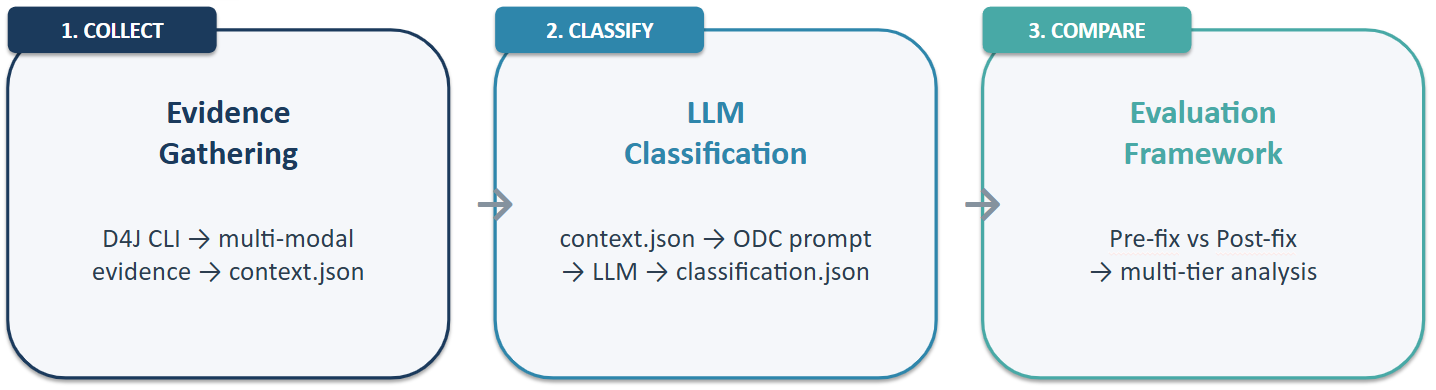
\includegraphics[width=0.95\linewidth]{pipeline_arch}
    \caption{Pipeline architecture overview showing the three stages: Collect, Classify, and Compare}
    \label{fig:pipeline_arch}
\end{figure}

Key architectural principles include multi-provider LLM support (Gemini, OpenRouter, OpenAI-compatible APIs), pre-fix evidence as the default mode, and hidden oracle exclusion where the list of modified classes never enters the LLM prompt to prevent data leakage. The design is inspired by AutoSD \cite{kang2023autosd}, which encoded Zeller's scientific debugging into an LLM pipeline for fault localization \cite{zeller2009why}.

\section{ODC and Defects4J Artifact Mapping}

The pipeline maps Defects4J artifacts to ODC attributes following the framework's two-phase opener/closer model, as shown in \autoref{fig:odc_d4j_mapping}.

\begin{figure}[H]
    \centering
    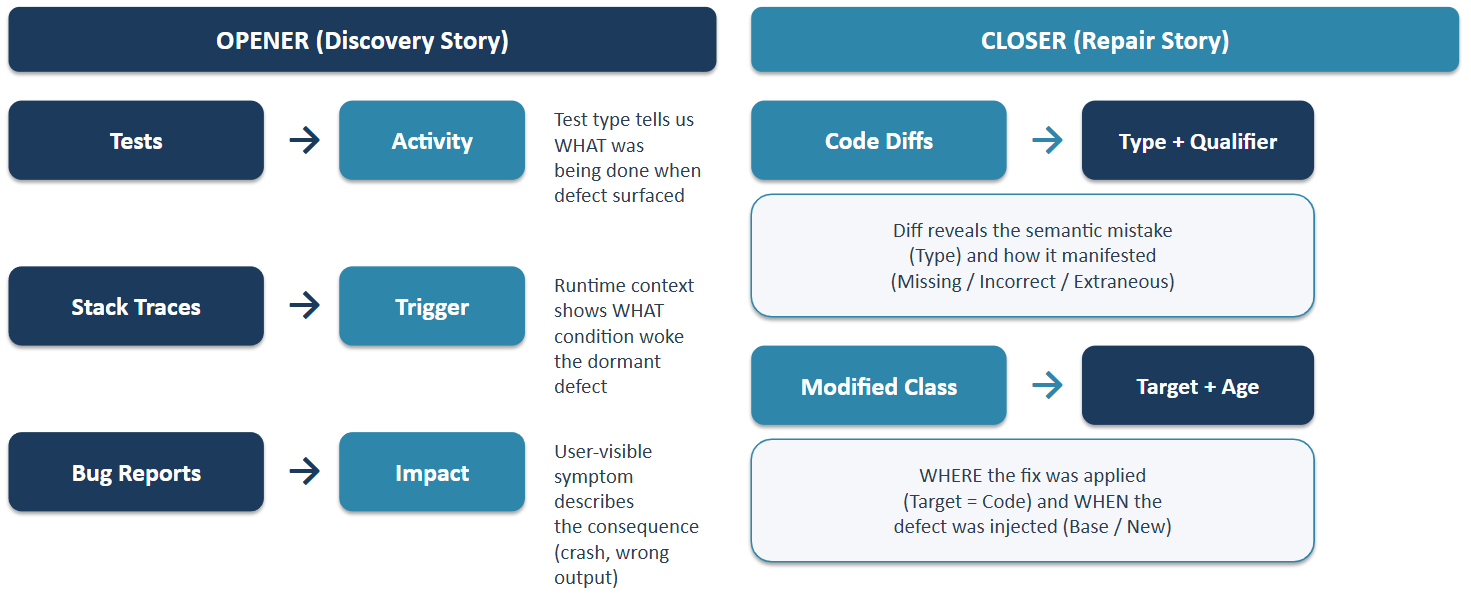
\includegraphics[width=0.95\linewidth]{odc_d4j_mapping}
    \caption{Natural mapping between Defects4J artifacts and ODC opener/closer attributes}
    \label{fig:odc_d4j_mapping}
\end{figure}

On the opener side (discovery story):
\begin{itemize}
    \item \textbf{Tests} map to \textbf{Activity}, because the test type (unit test, function test, system test) directly tells us what was being performed when the defect was found.
    \item \textbf{Stack Traces} map to \textbf{Trigger}, because the runtime context captured in the trace shows the specific condition that woke up the dormant defect.
    \item \textbf{Bug Reports} map to \textbf{Impact}, because they describe the user-visible symptom and consequence, such as a crash or wrong output.
\end{itemize}

On the closer side (repair story):
\begin{itemize}
    \item \textbf{Code Diffs} map to \textbf{Defect Type + Qualifier}, because the diff reveals the semantic nature of the mistake and how it manifested (Missing, Incorrect, or Extraneous).
    \item \textbf{Modified Classes} map to \textbf{Target + Age}, because they show where the fix was applied and when the defect was likely injected.
\end{itemize}

This clean separation ensures that subjective discovery data is never mixed with objective technical repair data, following ODC's fundamental design principle \cite{chillarege1992odc}.

\section{Evidence Collection}

The evidence collection stage gathers multi-modal bug information from Defects4J, as shown in \autoref{fig:evidence_collection}. The process follows eight sequential steps:

\begin{figure}[H]
    \centering
    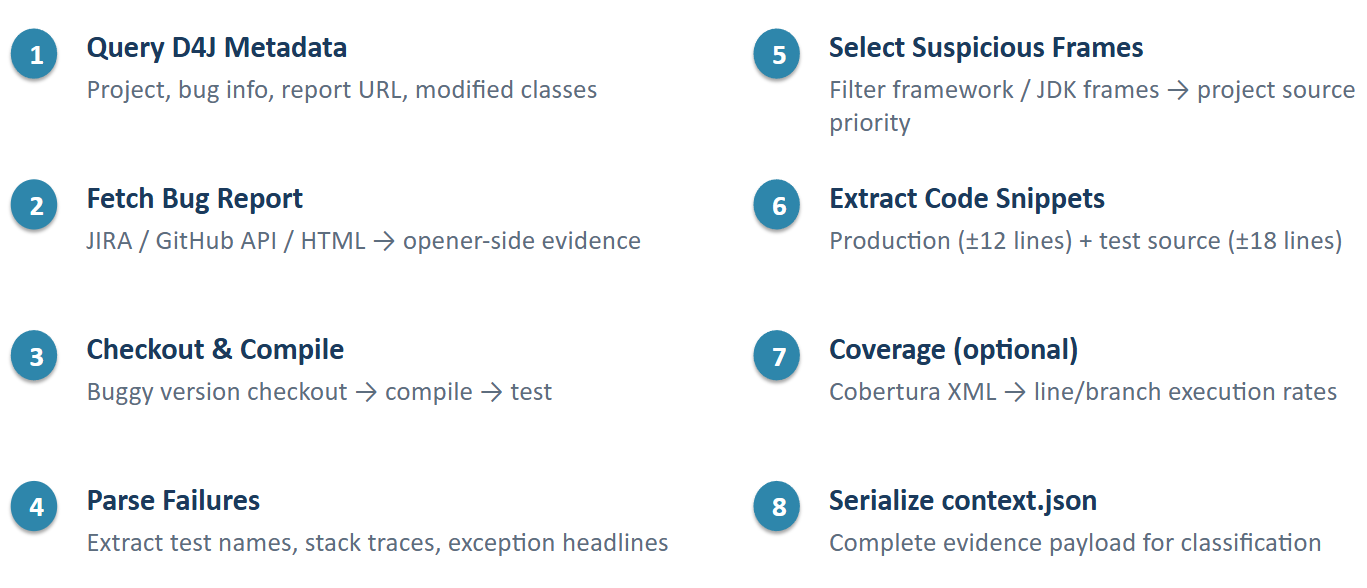
\includegraphics[width=0.95\linewidth]{evidence_collection}
    \caption{Evidence collection process: eight steps from metadata query to context serialization}
    \label{fig:evidence_collection}
\end{figure}

\begin{enumerate}
    \item \textbf{Query D4J Metadata:} Retrieve project information, bug details, and the report URL.
    \item \textbf{Fetch Bug Report:} Download the bug report content from JIRA, GitHub, or a generic web page for opener-side evidence.
    \item \textbf{Checkout and Compile:} Check out the buggy version and compile it.
    \item \textbf{Run Tests and Parse Failures:} Execute the test suite and extract test names, stack traces, and exception messages from the results.
    \item \textbf{Select Suspicious Frames:} Filter out framework, JDK, and build-tool frames, prioritizing project source code frames.
    \item \textbf{Extract Code Snippets:} Pull production code (plus or minus 12 lines around each suspicious frame) and test source code (plus or minus 18 lines) to show expected versus actual behavior.
    \item \textbf{Coverage (optional):} Run Cobertura-style coverage analysis and parse the resulting XML for line and branch execution rates.
    \item \textbf{Serialize context.json:} Package all collected evidence into a structured JSON file for the classification stage.
\end{enumerate}

An important design decision is hidden oracle exclusion: the list of modified classes (from \texttt{classes.modified}) is stored in a \texttt{hidden\_oracles} field and deliberately excluded from the LLM prompt to prevent data leakage \cite{rafi2024revisiting}.

\section{Evidence Modes: Pre-fix vs Post-fix}

The pipeline operates in two evidence modes to support both realistic classification and evaluation, as shown in \autoref{fig:prefix_postfix}.

\begin{figure}[H]
    \centering
    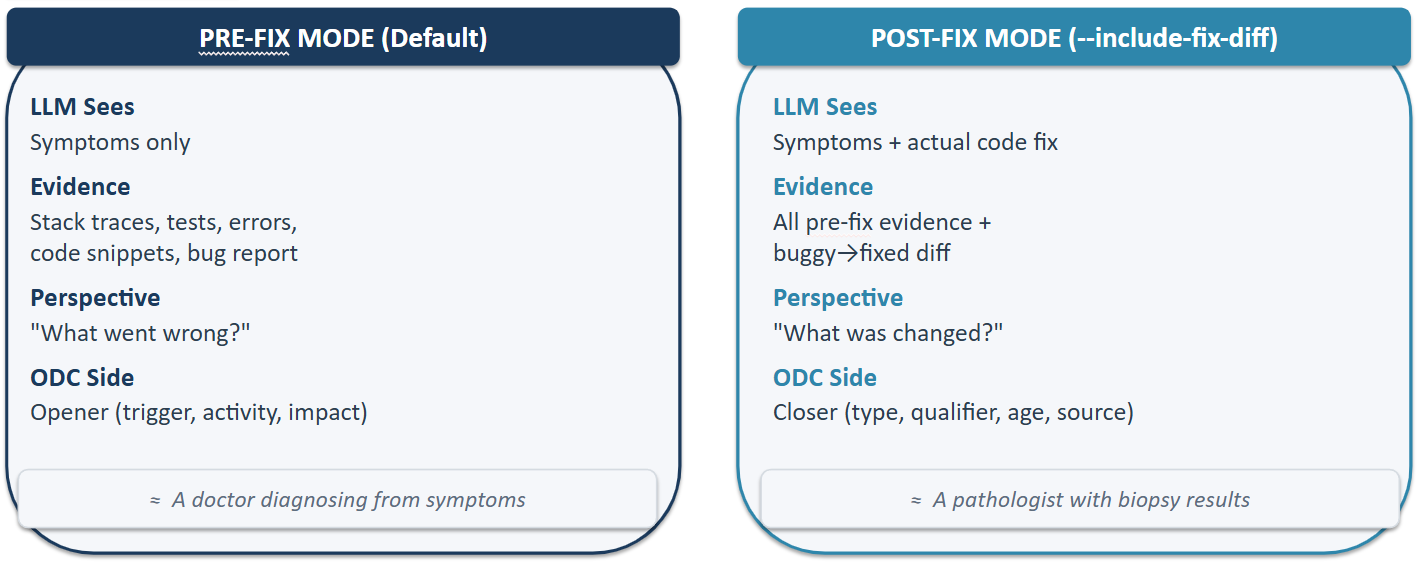
\includegraphics[width=0.95\linewidth]{prefix_postfix}
    \caption{Pre-fix vs Post-fix evidence modes with their corresponding ODC perspectives}
    \label{fig:prefix_postfix}
\end{figure}

\textbf{Pre-fix mode} (the default) gives the LLM only symptoms: stack traces, test failures, error messages, code snippets, and bug report content. The LLM sees what went wrong and must reason about the root cause without knowing the fix. This mirrors opener-side ODC evidence (trigger, activity, impact). Conceptually, this is like a doctor diagnosing a patient from symptoms alone.

\textbf{Post-fix mode} (enabled with the \texttt{--include-fix-diff} flag) adds the actual buggy-to-fixed code diff as oracle information. The LLM can now see exactly what was changed, giving it closer-side ODC evidence (defect type, qualifier, age, source). This is like a pathologist with biopsy results who can see the exact problem.

ODC's opener/closer model naturally requires evidence from both perspectives \cite{chillarege1992odc}. Pre-fix captures opener evidence, and post-fix captures closer evidence. This dual-mode design enables a built-in evaluation strategy: if the pipeline classifies correctly from symptoms alone, the pre-fix result should broadly agree with the post-fix result.

\section{Prompt Design}

The classification prompt consists of six components that work together to guide the LLM toward consistent, explainable ODC classifications. The prompt structure is shown in \autoref{fig:prompt_design}.

\begin{figure}[H]
    \centering
    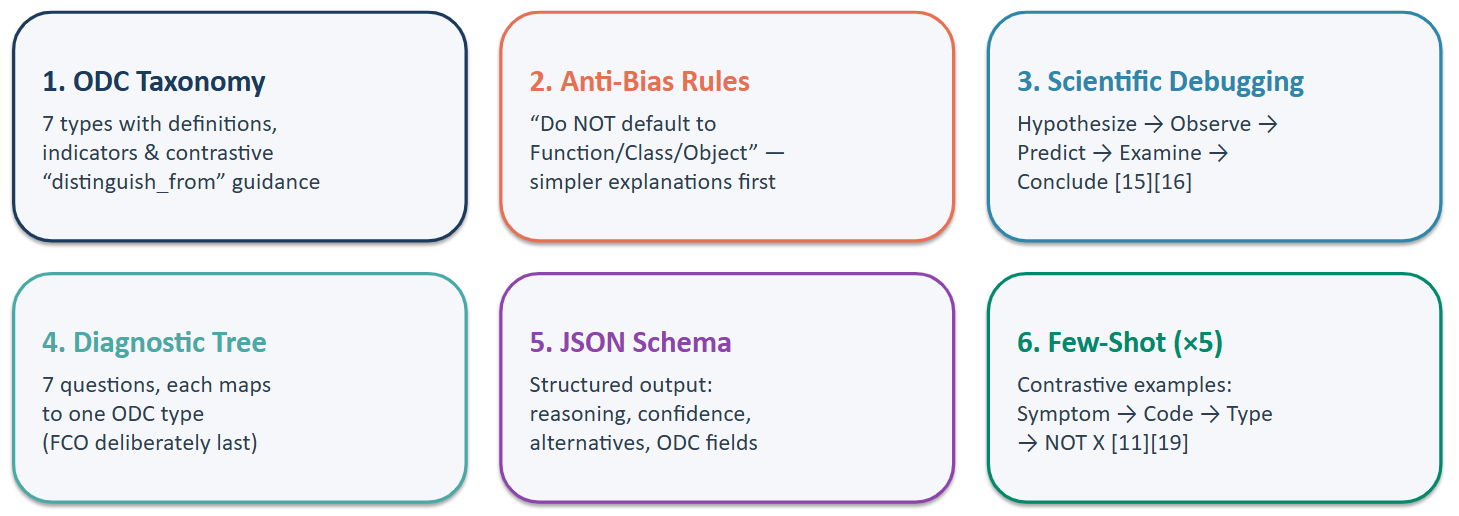
\includegraphics[width=0.95\linewidth]{prompt_design}
    \caption{Six components of the system prompt: ODC taxonomy, anti-bias rules, scientific debugging, diagnostic tree, JSON schema, and few-shot examples}
    \label{fig:prompt_design}
\end{figure}

\begin{enumerate}
    \item \textbf{ODC Taxonomy:} The seven defect types with definitions, diagnostic indicators, and contrastive ``distinguish from'' guidance that helps the LLM differentiate between similar types.
    \item \textbf{Anti-Bias Rules:} Explicit instructions to avoid defaulting to Function/Class/Object, which is the most general structural type. The prompt forces the LLM to consider simpler explanations first.
    \item \textbf{Scientific Debugging Protocol:} A structured five-step process (Hypothesize, Observe, Predict, Examine, Conclude) based on Zeller's scientific debugging methodology \cite{zeller2009why}, adapted for LLM prompting following the approach of \textcite{kang2023autosd}.
    \item \textbf{Diagnostic Decision Tree:} Seven questions, each mapping to one ODC type. Function/Class/Object is deliberately placed last to force consideration of simpler types first \cite{nong2024cot}.
    \item \textbf{JSON Schema:} A structured output format that requires reasoning traces, confidence scores, alternative type considerations, and ODC attribute fields.
    \item \textbf{Few-Shot Examples (5):} Contrastive examples that demonstrate the pattern: Symptom, Code, Classification, and why it is NOT another type \cite{koyuncu2025exploring}.
\end{enumerate}

\section{Scientific Debugging Protocol}

The scientific debugging protocol is the core reasoning strategy encoded into the LLM prompt. It adapts Zeller's five-step scientific debugging approach \cite{zeller2009why} for ODC classification, as shown in \autoref{fig:scientific_debug}.

\begin{figure}[H]
    \centering
    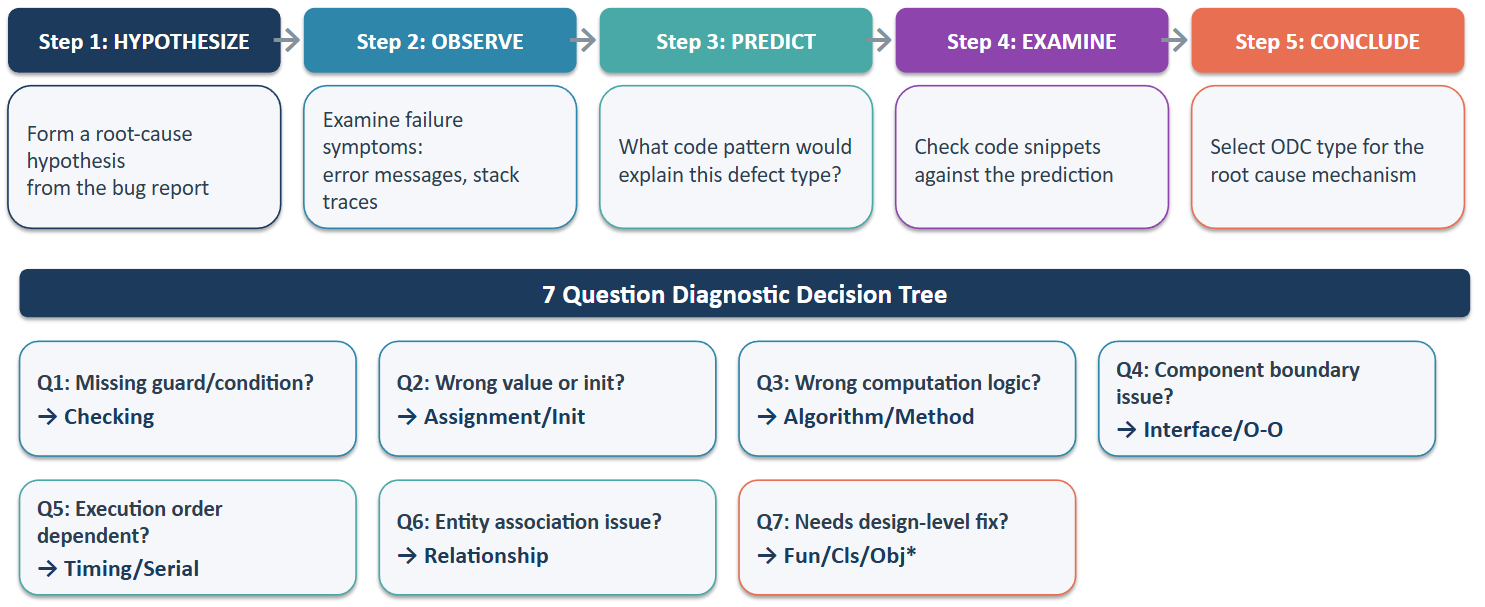
\includegraphics[width=0.95\linewidth]{scientific_debug}
    \caption{Scientific debugging protocol with five steps and the 7-question diagnostic decision tree}
    \label{fig:scientific_debug}
\end{figure}

The five steps are:
\begin{enumerate}
    \item \textbf{Hypothesize:} Form a root-cause hypothesis from the bug report.
    \item \textbf{Observe:} Examine failure symptoms including error messages and stack traces.
    \item \textbf{Predict:} Determine what code pattern would explain this defect type.
    \item \textbf{Examine:} Check code snippets against the prediction.
    \item \textbf{Conclude:} Select the ODC type that best explains the root cause mechanism.
\end{enumerate}

The diagnostic decision tree consists of seven questions (Q1 through Q7), each corresponding to one ODC type. Q7 (``Does this need a design-level fix?'') is deliberately placed last because Function/Class/Object should only be selected when all simpler types have been ruled out. This ordering was inspired by the anti-bias principles in chain-of-thought prompting research \cite{nong2024cot}.

\section{Classification Pipeline and Validation}

The classification stage takes a \texttt{context.json} file and produces a \texttt{classification.json} file through a structured process, as shown in \autoref{fig:classification_flow}.

\begin{figure}[H]
    \centering
    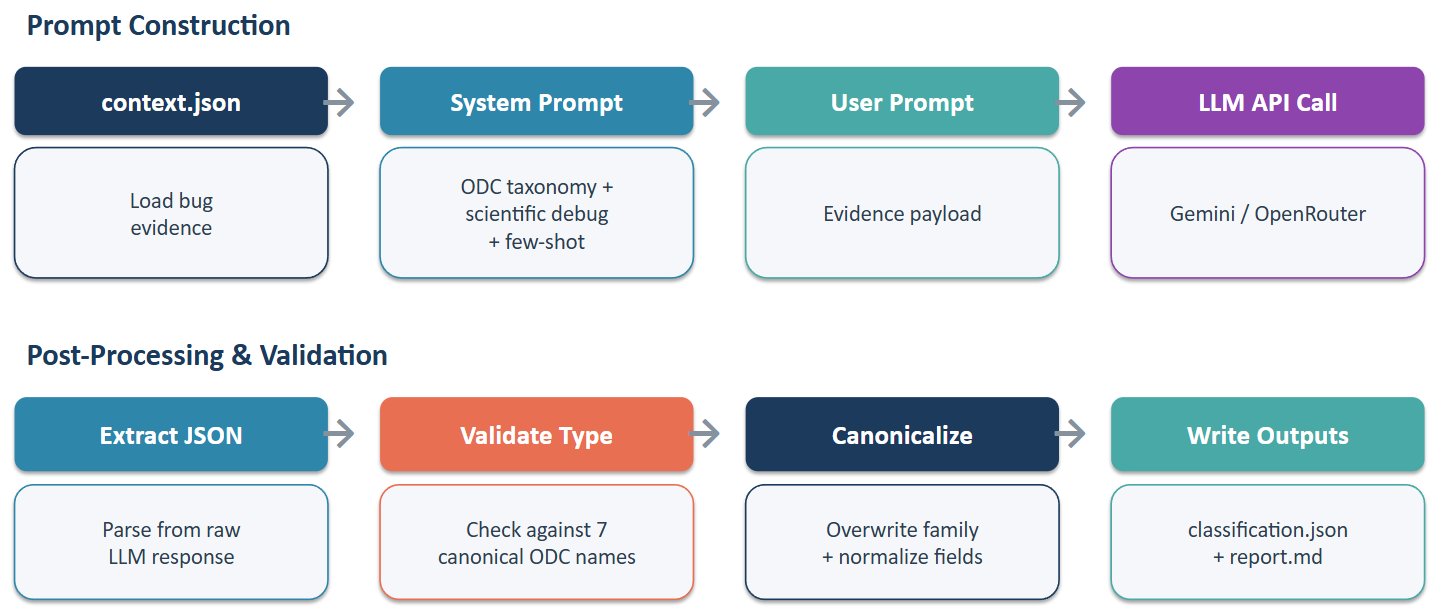
\includegraphics[width=0.95\linewidth]{classification_flow}
    \caption{Classification pipeline flow from context loading through validation to output}
    \label{fig:classification_flow}
\end{figure}

The process consists of:
\begin{enumerate}
    \item \textbf{Prompt Construction:} Load the bug evidence, build the system prompt (ODC taxonomy + scientific debugging + few-shot examples), and construct the user prompt (evidence payload with hidden oracles filtered out).
    \item \textbf{LLM API Call:} Send the prompt to the configured LLM provider (Gemini, OpenRouter, or OpenAI-compatible).
    \item \textbf{Response Parsing:} Extract the JSON classification from the raw LLM response, handling fenced code blocks and extra text.
    \item \textbf{ODC Validation:} Validate the \texttt{odc\_type} against the canonical seven types. The family is always recomputed from the type (not trusted from the model) to ensure consistency.
    \item \textbf{Output Generation:} Write the validated \texttt{classification.json} and optionally generate a human-readable \texttt{report.md}.
\end{enumerate}

The pipeline supports multi-provider LLM backends. Gemini uses a response JSON schema for structured output, while OpenRouter and OpenAI-compatible providers use chat completions with post-hoc JSON parsing. Transient HTTP errors (429, 500, 502, 503) are retried with exponential backoff.

\section{Evaluation Framework}

The pipeline uses a 4-tier evaluation framework to compare pre-fix and post-fix classifications, as shown in \autoref{fig:eval_framework}. This multi-tier approach is necessary because even human ODC experts disagree on 20 to 30\% of bugs \cite{chillarege1992odc}.

\begin{figure}[H]
    \centering
    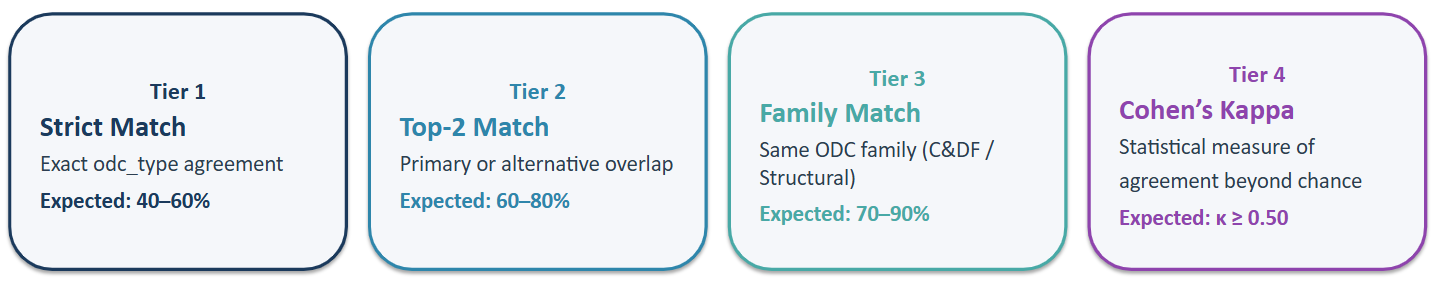
\includegraphics[width=0.95\linewidth]{eval_framework}
    \caption{4-tier evaluation framework: Strict Match, Top-2 Match, Family Match, and Cohen's Kappa}
    \label{fig:eval_framework}
\end{figure}

The four tiers are:
\begin{enumerate}
    \item \textbf{Strict Match:} Do the pre-fix and post-fix classifications assign the exact same ODC type? This is the most demanding metric.
    \item \textbf{Top-2 Match:} Is the pre-fix primary type found in the post-fix alternative types (or vice versa)? This captures cases where the LLM correctly identified the type but ranked it second.
    \item \textbf{Family Match:} Do both classifications fall within the same family (Control and Data Flow or Structural)? This captures broad semantic agreement even when the specific type differs.
    \item \textbf{Cohen's Kappa:} A statistical measure of inter-rater reliability that accounts for chance agreement, computed only in batch comparisons \cite{thung2012automatic}.
\end{enumerate}

This tiered approach captures both exact agreement and meaningful near-agreement, matching industry evaluation practice \cite{chillarege1992odc, thung2012automatic}.

\section{Summary}

The proposed methodology combines three ideas: multi-modal evidence from Defects4J, ODC's principled taxonomy, and Zeller's scientific debugging protocol, all encoded into structured LLM prompts. The dual-mode (pre-fix/post-fix) design provides a built-in evaluation mechanism, and the 4-tier comparison framework respects the inherent ambiguity in defect classification. The next chapters describe the experimental setup and preliminary results from applying this methodology.


% ================================================================
% CHAPTER 5: EXPERIMENTAL DESIGN / DATA COLLECTION PLAN
% ================================================================
\chapter{Experimental Design and Data Collection}

This chapter describes how we set up our experiments, what data we collected, and how we configured the pipeline for the classification runs.

\section{Dataset: Defects4J}

The experiment uses the Defects4J benchmark dataset version 2.0, which contains over 864 active bugs across 17 open-source Java projects \cite{just2014defects4j}. \autoref{tab:d4j_projects} shows the projects included in the dataset.

\begin{table}[H]
    \centering
    \begin{tabular}{l l r}
        \toprule
        \textbf{Project} & \textbf{Description} & \textbf{Active Bugs} \\
        \midrule
        Chart & JFreeChart plotting library & 26 \\
        Cli & Apache Commons CLI & 40 \\
        Closure & Google Closure Compiler & 174 \\
        Codec & Apache Commons Codec & 18 \\
        Collections & Apache Commons Collections & 4 \\
        Compress & Apache Commons Compress & 47 \\
        Csv & Apache Commons CSV & 16 \\
        Gson & Google Gson & 18 \\
        JacksonCore & Jackson JSON core & 26 \\
        JacksonDatabind & Jackson databinding & 112 \\
        JacksonXml & Jackson XML & 6 \\
        Jsoup & HTML parser & 93 \\
        JxPath & Apache JXPath & 22 \\
        Lang & Apache Commons Lang & 64 \\
        Math & Apache Commons Math & 106 \\
        Mockito & Mocking framework & 38 \\
        Time & Joda-Time & 26 \\
        \midrule
        \textbf{Total} & & \textbf{835+} \\
        \bottomrule
    \end{tabular}
    \caption{Defects4J projects and their active bug counts}
    \label{tab:d4j_projects}
\end{table}

Each bug provides the following artifacts used by our pipeline: bug reports (from JIRA, GitHub, or project trackers), triggering test cases, buggy source code, fixed source code, and buggy-to-fixed diffs. Defects4J also provides CLI tools for checkout, compilation, test execution, and coverage analysis.

\section{Experimental Setup}

\subsection{Evidence Collection Configuration}

For each bug, the pipeline collects evidence in two modes:
\begin{itemize}
    \item \textbf{Pre-fix:} Symptoms only (bug reports, stack traces, failing tests, code snippets). No access to the fix.
    \item \textbf{Post-fix:} All pre-fix evidence plus the actual buggy-to-fixed code diff (enabled with \texttt{--include-fix-diff}).
\end{itemize}

Stack frame filtering is configured to remove framework frames (JUnit, TestNG, Hamcrest), JDK internal frames, and build-tool frames. Only project source frames are retained. Production code snippets capture plus or minus 12 lines around each suspicious frame. Test source snippets capture plus or minus 18 lines and are capped at the first 3 failing tests.

\subsection{LLM Configuration}

The classification uses the scientific prompt style with the following LLM configuration:
\begin{itemize}
    \item \textbf{Provider:} Google Gemini (primary), with OpenRouter as secondary
    \item \textbf{Prompt style:} Scientific (includes the 5-step debugging protocol and 7-question decision tree)
    \item \textbf{Few-shot examples:} 5 contrastive examples included in every prompt
    \item \textbf{Output format:} Structured JSON with reasoning traces, confidence scores, and alternative type considerations
\end{itemize}

\subsection{Evaluation Configuration}

Each bug produces two classification files: one from pre-fix evidence and one from post-fix evidence. The \texttt{compare-batch} command automatically discovers matching pairs and computes all four evaluation tiers (strict match, top-2 match, family match, and Cohen's Kappa).

\section{Data Collection Plan}

The full experiment targets all 864+ active Defects4J bugs. For the preliminary analysis presented in this report, we have completed 34 bug pairs across 17 projects. The full dataset run is planned as a batch operation covering all remaining bugs.

The data collection process for each bug follows these steps:
\begin{enumerate}
    \item Run \texttt{d4j-odc collect} to generate pre-fix \texttt{context.json}
    \item Run \texttt{d4j-odc classify} on the pre-fix context
    \item Run \texttt{d4j-odc collect --include-fix-diff} to generate post-fix \texttt{context.json}
    \item Run \texttt{d4j-odc classify} on the post-fix context
    \item Run \texttt{d4j-odc compare} to evaluate the pair
\end{enumerate}

After all individual pairs are processed, \texttt{compare-batch} aggregates the results and computes dataset-wide statistics.

\section{Multi-Fault Context}

An important consideration for evaluation is that Defects4J bugs do not exist in isolation. Research by \textcite{callaghan2024mf} shows that real programs average approximately 9.2 co-existing faults per version. Our pipeline includes a multi-fault awareness module that can query the defects4j-mf dataset to identify how many other faults co-exist with each bug. This context helps explain classification divergence in cases where symptom evidence is contaminated by multiple overlapping faults.


% ================================================================
% CHAPTER 6: EXPECTED RESULTS
% ================================================================
\chapter{Results and Analysis}

This chapter presents the preliminary results from our analysis of 34 bug pairs across 17 Defects4J projects and discusses their implications.

\section{Classification Results Overview}

The preliminary analysis of 34 pre-fix vs post-fix classification pairs produces the following results across the 4-tier evaluation framework, as shown in \autoref{tab:eval_results}.

\begin{table}[H]
    \centering
    \begin{tabular}{l r r}
        \toprule
        \textbf{Evaluation Tier} & \textbf{Match Count} & \textbf{Rate} \\
        \midrule
        Strict Match (exact same type) & 25/34 & 73.5\% \\
        Top-2 Match (including alternatives) & 32/34 & 94.1\% \\
        Family Match (same family) & 33/34 & 97.1\% \\
        \bottomrule
    \end{tabular}
    \caption{Preliminary evaluation results across the 4-tier framework (34 bug pairs)}
    \label{tab:eval_results}
\end{table}

These results show that while the exact type does not always match between pre-fix and post-fix classifications, the disagreement is almost always within the same family of defect types. The 73.5\% strict match rate is consistent with ODC literature, which reports that even human experts disagree on 20 to 30\% of defect classifications \cite{chillarege1992odc}.

\section{Analysis of Type-Shifted Bugs}

Out of 34 bug pairs, 9 showed a type shift (different ODC type between pre-fix and post-fix). Of these 9:
\begin{itemize}
    \item 7 bugs showed cross-alternative overlap, meaning the pre-fix primary type appeared in the post-fix alternative types or vice versa. This indicates that the LLM identified the correct type but ranked it differently depending on available evidence.
    \item 2 bugs (JacksonCore-24 and Math-34) showed no alternative overlap, but both still matched at the family level.
\end{itemize}

This pattern is expected and scientifically explainable. Pre-fix classification works from symptoms (like a doctor diagnosing from symptoms), while post-fix classification works from the actual fix (like a pathologist with biopsy results). The two perspectives naturally emphasize different aspects of the same underlying defect.

\section{Why Types Diverge}

The 26.5\% type-shift rate reflects the expected difference between symptom-based and cause-based classification, not a failure of the pipeline. Three main factors explain why pre-fix and post-fix classifications can disagree:

\begin{enumerate}
    \item \textbf{Evidence Asymmetry:} Pre-fix evidence shows symptoms (what went wrong), while post-fix evidence shows the cause (what was changed). Symptoms and causes can suggest different ODC types because a single root cause can produce multiple different symptoms.
    \item \textbf{ODC Boundary Ambiguity:} Some bugs legitimately sit near the boundary between two ODC types. For example, a missing null check could be classified as either Checking (the validation was absent) or Algorithm/Method (the computation should have handled null inputs). Which type the LLM selects depends on whether it sees only the symptom or the fix.
    \item \textbf{Multi-Fault Context:} Defects4J programs contain an average of 9.2 co-existing faults per version \cite{callaghan2024mf}. When multiple faults co-exist, symptom evidence from one fault can contaminate the classification of another.
\end{enumerate}

The 97.1\% family match demonstrates that even when the specific type shifts, the pipeline consistently identifies the correct broad category of defect. This shows robust semantic consistency in the classification approach \cite{chillarege1992odc, thung2012automatic}.

\section{Project Coverage}

The preliminary 34 bugs span 17 Defects4J projects, providing initial coverage across the full project spectrum. The distribution of bugs per project in this sample is not uniform, as we prioritized diversity across projects over depth within any single project for the initial analysis. The full experiment will cover all active bugs in every project.

\section{Summary}

The preliminary results demonstrate that the pipeline produces semantically consistent classifications. The 73.5\% strict match, 94.1\% top-2 match, and 97.1\% family match rates fall well within the expected range for ODC classification, where perfect agreement is neither expected nor required. The type-shift patterns are scientifically explainable through evidence asymmetry, ODC boundary ambiguity, and multi-fault contamination.


% ================================================================
% CHAPTER 7: PROJECT TIMELINE
% ================================================================
\chapter{Project Timeline}

This chapter presents the timeline for our research project, from initial literature review through final thesis submission. \autoref{tab:timeline} summarizes the major phases and their planned durations.

\begin{table}[H]
    \centering
    \begin{tabular}{r l l}
        \toprule
        \textbf{Phase} & \textbf{Activity} & \textbf{Duration} \\
        \midrule
        1 & Literature review and ODC study & Weeks 1--4 \\
        2 & Pipeline architecture design & Weeks 3--5 \\
        3 & Evidence collection module & Weeks 5--8 \\
        4 & LLM classification module & Weeks 7--10 \\
        5 & Prompt engineering and tuning & Weeks 9--12 \\
        6 & Evaluation framework and comparison & Weeks 11--13 \\
        7 & Preliminary experiments (34 bugs) & Weeks 12--14 \\
        8 & Full dataset classification run & Weeks 14--18 \\
        9 & Results analysis and discussion & Weeks 17--19 \\
        10 & Thesis writing and revision & Weeks 16--22 \\
        11 & Pre-defense presentation & Week 22 \\
        12 & Final thesis submission & Week 24 \\
        \bottomrule
    \end{tabular}
    \caption{Project timeline with overlapping phases}
    \label{tab:timeline}
\end{table}

Phases 1 through 7 have been completed. We are currently in Phase 8 (full dataset run) and Phase 10 (thesis writing) concurrently. The overlapping phases reflect the iterative nature of the research, where prompt engineering improvements discovered during experiments feed back into the pipeline design.


% ================================================================
% CHAPTER 8: CONCLUSION
% ================================================================
\chapter{Conclusion}

This chapter summarizes our work, discusses its limitations, and outlines future research directions.

\section{Summary}

This thesis presents an automated pipeline for classifying Defects4J bugs into Orthogonal Defect Classification (ODC) defect types using Large Language Model reasoning guided by a scientific debugging protocol. The key contributions are:

\begin{enumerate}
    \item An end-to-end pipeline that collects multi-modal evidence from Defects4J artifacts and produces machine-readable ODC classifications with full reasoning traces.
    \item A dual-mode evidence system (pre-fix and post-fix) that mirrors ODC's opener/closer model and enables built-in evaluation.
    \item A structured prompting approach that combines ODC taxonomy constraints with Zeller's scientific debugging methodology.
    \item A 4-tier evaluation framework that measures classification agreement at multiple granularity levels.
\end{enumerate}

Preliminary results from 34 bug pairs show 73.5\% strict match, 94.1\% top-2 match, and 97.1\% family match, demonstrating that the pipeline produces semantically consistent classifications that fall within the expected range for ODC expert agreement.

\section{Limitations}

The current work has several limitations that should be considered:

\begin{itemize}
    \item \textbf{LLM Reproducibility:} Different LLM providers and model versions may produce different classifications for the same bug. Temperature settings and model updates can affect consistency across runs.
    \item \textbf{Single-Model Classification:} The current pipeline uses a single LLM for each classification. There is no consensus mechanism across multiple models or multiple runs of the same model.
    \item \textbf{No Ground-Truth Labels:} Since Defects4J does not include human-labeled ODC types, there is no external ground truth to validate individual classifications against. Our evaluation relies on pre-fix vs post-fix agreement as a proxy for correctness.
    \item \textbf{Java Only:} The pipeline is designed specifically for Defects4J, which contains only Java projects. Extending to other programming languages or bug datasets would require adaptation of the evidence collection module.
    \item \textbf{Partial Dataset Coverage:} The preliminary results cover only 34 bugs. The full 864+ bug analysis is still in progress.
\end{itemize}

\section{Future Work}

Several research directions could extend and improve this work:

\begin{itemize}
    \item \textbf{Multi-Model Consensus:} Running multiple LLMs or multiple runs on the same bug and using voting or aggregation to produce more reliable classifications \cite{colavito2024llm}.
    \item \textbf{Cross-Language Extension:} Adapting the pipeline to work with other bug benchmark datasets beyond Defects4J, covering different programming languages and project types.
    \item \textbf{Automated Program Repair Integration:} Using ODC classifications to select and guide appropriate repair strategies, connecting the classification output to automated program repair tools \cite{durieux2018automatic}.
    \item \textbf{Longitudinal Process Analysis:} Studying how ODC type distributions change over time within a project to identify quality trends and process improvements \cite{catolino2019not}.
    \item \textbf{Human Expert Validation:} Conducting a formal study where human ODC experts label a subset of Defects4J bugs to create a ground-truth validation set for the pipeline.
\end{itemize}

\section{Closing Remarks}

Defect classification is a fundamental building block of software quality assurance. By combining the rigor of ODC's taxonomy with the reasoning capabilities of modern LLMs and the structure of scientific debugging, this thesis provides a practical, scalable approach to a problem that has traditionally required expensive manual analysis. The preliminary results suggest that LLM-driven ODC classification is a viable and promising direction for making bug triage faster, more consistent, and more informative.


%-------------------------- BACK MATTER --------------------------%

\printbib

\end{document}
